\documentclass[twocolumn]{aastex62}

\usepackage[utf8]{inputenc}
\usepackage{url}
\usepackage{minted}
\usepackage{xspace}
\usepackage{natbib}  % Requires natbib.sty, available from http://ads.harvard.edu/pubs/bibtex/astronat/

\newcommand{\pyspeckit}{\texttt{pyspeckit}\xspace}
\newcommand{\astropy}{\texttt{astropy}\xspace}
\begin{document}

\title{pyspeckit}
%\authorrunning{Ginsburg et al}

\author[0000-0001-6431-9633]{Adam Ginsburg}
%\nraojansky


\begin{abstract}
\pyspeckit is a tool and library for spectroscopic analysis in Python. We describe the
\pyspeckit package and highlight some of its unique capabilities such as
interactively fitting a model to data, akin to the widely-used \texttt{splot} function
of \texttt{IRAF}. \pyspeckit employs the Levenberg-Marquardt optimization method 
via \texttt{mpfit} and \texttt{lmfit}, and important assumptions regarding error estimation 
are described here. Wrappers for \texttt{pymc} and \texttt{emcee} are available, as well as a 
method to fit lines in spectral cubes. As part of the \astropy affiliated packages, 
\pyspeckit is open source and welcomes input and collaboration from the community.
\end{abstract}


\section{Introduction}
Spectroscopy is an important tool for astronomy, and we seek to enable Python users
to quickly and easily analyze spectra.  Spectra are represented as
the number of photons, or total energy in photons, arriving over a specified
wavelength (or equivalently, frequency or energy) range. Emission and 
absorption lines due to ions, atoms, and molecules bear important information
via their line flux, line width, and velocity centroid. These parameters are
typically measured from model fits to the data, such as Gaussians, Lorentzians,
and Voigt profiles. Historically, \texttt{IRAF} has provided the astronomy
community with easy-to-use tools for line fittings, but \texttt{IRAF}
development has mostly ceased in the last several years and is currently only
supported in Python 2.7 by
AstroConda\footnote{http://astroconda.readthedocs.io/en/latest/index.html},
though the PyRAF command language supports both Python 2 and Python 3 and is
still maintained.

[It would be interesting to describe the history and purpose of \pyspeckit and \astropy here] 
Development of \pyspeckit began several years before \astropy began...  Several
features were therefore implemented that were later replaced by similar
\astropy features, in particular the unit system.  Unit conversions in
\pyspeckit are now (as of October 2015) done entirely using the \astropy
system...

In this paper we briefly outline \texttt{pyspeckit} architecture and highlight its key 
capabilities. In Section XX...



\section{Basic structure}
The central object in \pyspeckit is a \texttt{Spectrum} object, which has
associated \texttt{data} (e.g., flux), \texttt{error}, and \texttt{xarr} (e.g., wavelength,
frequency, energy), the latter of
which represents the spectroscopic axis.  A \texttt{Spectrum} object has
several attributes that are themselves sophisticated classes that can be called
as functions: the \texttt{plotter}, the fitter \texttt{specfit}, and the
continuum fitter \texttt{baseline}.

There are several important subclasses of \texttt{Spectrum}: \texttt{Spectra}
is a collection of spectra intended to be stitched together (i.e., with
non-overlapping spectral axes), \texttt{ObsBlock} is a collection of spectra
with identical spectral axes intended to be operated on as a group, e.g., to
take an average spectrum, and \texttt{Cube} is a 3D spatial-spatial-spectral
cube.

\subsection{Supported data formats}

\pyspeckit{} supports a variety of open and proprietary data formats that have
been traditionally used to store spectral data products in astronomy.  Reading
a one-dimensional spectrum from a text file with an optional error column can
be done using the \texttt{astropy.io.ascii} module in any of its supported
formats.  The Flexible Image Transport System \citep[FITS;][]{Pence2010a} format is
supported in \pyspeckit{} with \texttt{astropy.io.fits}.  Initially developed
by optical astronomers, the FITS standard has incorporated several
recommendations for various types of data formats used in the astronomy
community into successive updates to the standard---the latest version of the
standard being 4.0 from 2016.  Additionally, data files following the Single
Dish FITS \citep[SDFITS;][]{Garwood2000a} convention for radio astronomy data as
produced by the Green Bank Telescope are partially supported in \pyspeckit.
The Hierarchical Data Format (HDF5) file format has been designed to store and
organize large amounts of data and offers significant advantages over FITS\@.
Although not widely used in observational astronomy, the pipeline of the
Low-Frequency Array (LOFAR) radio telescope uses the HDF5 data format to
efficiently store large data volumes \citep{Alexov2012a}.  If the \texttt{h5py}
package is installed, \pyspeckit{} will support read access to files containing
spectra in the HDF5 format (although there is no specified standard for spectra in
HDF5).  Finally, \pyspeckit{} is capable of reading files
from some versions of the GILDAS Continuum and Line Analysis Single-dish
Software format \citep[CLASS;][]{Gildas-Team2013a}.  Since the CLASS file specification
is incomplete and will remain private for the foreseeable future, much of the
data reading in \pyspeckit{} has been reproduced in an approximate manner.  The
CLASS reader is known to work well with data files from the Arizona Radio
Observatory telescopes (12-m and 10-m Submillimeter Telescope) and the Atacama
Pathfinder Experiment (APEX) radio telescope.

\subsection{Plotter}
The plotter is a basic line plotter.  See the GUI section (\S \ref{sec:gui})
for more details.

% Should we include code examples of how to do these things? I think examples
% creating a Spectrum, plotting it, interactively fitting, and then 
% printing out parinfo on the command line would be neat.

\subsection{Fitter}
\label{sec:fitters}
The fitting tool in \pyspeckit is the \texttt{Spectrum.specfit} object.
This object is a class that is created for every \texttt{Spectrum} object.
The fitter can be used with any of the models included in the model
registry, or a custom model can be created and registered.

To fit a profile to a spectrum, several optimizers are available.  Two
implementations of the Levenberg-Marquardt optimization method
\citep{Levenberg1944a,Marquardt1963a} are provided,
\texttt{mpfit}\footnote{Originally implemented by Craig Markwardt
\url{https://www.physics.wisc.edu/~craigm/idl/fitqa.html} and ported to python
by Mark Rivers and then Sergei Koposov.  The version in pyspeckit has been
updated somewhat from Koposov's version.} and
\texttt{lmfit}\footnote{\url{https://lmfit.github.io/lmfit-py/},
\url{http://dx.doi.org/10.5281/zenodo.11813}}.  Wrappers of
\texttt{pymc}\footnote{\url{https://pymc-devs.github.io/pymc/}} and
\texttt{emcee}\footnote{\url{http://dfm.io/emcee/current/},
\citet{Foreman-Mackey2013a}} are also available, though these tools are better
for parameter error analysis than for optimization.

Once a fit is performed, the results of the fit are accessible through the
\texttt{parinfo} object, which is a dictionary-like structure containing
the parameter values, errors, and other metadata (e.g., information about
whether the parameter is fixed, tied to another parameter, or limited).
Other information about the fit, such as the $\chi^2$ value, are available
as attributes of the \texttt{specfit} object.

\paragraph{Optimal $\chi^2$}
There is a tool to compute the `optimal' $\chi^2$, which is the $\chi^2$
value computed only over the range where the model contains statistically
significant signal.  By default, the function selects all pixels where
the model value is greater (in absolute value) than the corresponding error.
In principle, this optimal $\chi^2$ may be helpful for obtaining correctly
scaled errors (see Section \ref{sec:parerrest}), though this claim has never
been rigorously tested.


\subsection{Error Treatment}
%(Can I refer back to anything here?  like, "Error estimation is an important part of astronomy...")
%(the next two paragraphs may be redundant)

%The basic approach to fit a spectrum is to assign an error to each pixel in the
%\texttt{data} array by providing a value in the \texttt{sp.error} array.  These
%values are assumed to be $1-\sigma$ Gaussian errors on the data.


The \texttt{Spectrum} objects used by pyspeckit have an attached \texttt{error}
array, which is meant to hold the $1-\sigma$ independent Gaussian errors on
each pixel.  While this error representation may be a dramatic
oversimplification of the true errors for almost all instruments (since it
completely ignores correlation between adjacent pixels), it is also the most
commonly used assumptions in most astronomical applications.

The errors are used to determine the best-fit parameters and their errors (see
\S \ref{sec:fitters}).  They can be displayed as error bars on individual
pixels or as shaded regions around those pixels using different display modes

A typical example is given below, where we generate a spectrum and error
array using \texttt{numpy} and \texttt{astropy} tools.

\begin{minipage}{\linewidth}
\begin{minted}{python}
from astropy import units as u
import numpy as np
import pyspeckit

xaxis = np.linspace(-25, 25)*u.km/u.s
sigma = 3.0*u.km/u.s
data = 5*np.exp(-xaxis**2 /
                (2*sigma**2))*u.Jy
error = np.ones_like(data) * 0.2
sp = pyspeckit.Spectrum(xarr=xaxis,
                        data=data,
                        error=error)

sp.plotter(errstyle='fill')

sp.plotter.savefig("example_fig_1.pdf")
\end{minted}
\end{minipage}

\begin{figure*}[!htp]
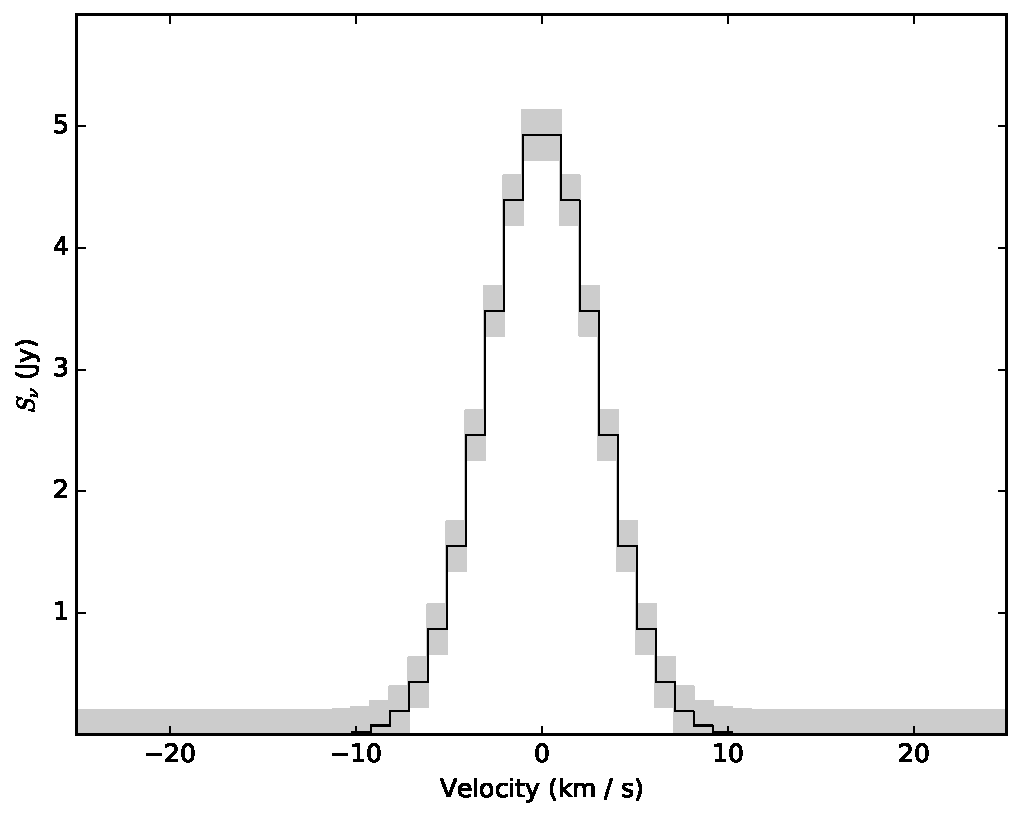
\includegraphics[scale=1,width=4in]{example_fig_1.pdf}
\caption{An example plotted spectrum showing the automated unit labeling
and errors.  The errors are shown with the \texttt{`fill'} style
and represent symmetric 1-$\sigma$ Gaussian errors.  }
\label{fig:example1}
\end{figure*}




\subsubsection{Automatic Error Estimation}
If a \texttt{Spectrum} is created with no associated errors, \pyspeckit can automatically
estimate the errors from a fit residual. When a fit is initiated on a \texttt{Spectrum}
with no specified errors, the errors will default to being uniformly 1.0. Uniform
weighting for each data point is likely not accurate, but will result in the appropriate 
best-fit parameters with \emph{incorrect} errors.

One common approach in spectroscopy in the limit that there are few pixels with
signal and many pixels representing only noise is to estimate the errors by the
standard deviation of the signal-free pixels.  This approach generally assumes
the noise is constant across the spectrum.  In the case that a single signal
feature is present in the spectrum, and it can be accurately modeled, the
standard deviation of the residual spectrum from the model fit will accurately
represent the uniform errors.  \pyspeckit will automatically replace the errors
with the standard deviation of the residuals if a fit is performed with
uninitialized errors; this means that performing a fit on the same data
(without associated errors) twice will result in the same parameter values both
times, but different errors the second time.


\subsubsection{Parameter error estimation}
\label{sec:parerrest}
Parameter errors are adopted from the \texttt{mpfit} or \texttt{lmfit}
fit results.  The Levenberg-Marquardt algorithm
 finds a local minimum in parameter space,
and one of its returns is the parameter covariance matrix.  This covariance
matrix is not directly the covariance of the parameters, and must be rescaled
to deliver an approximate error.

The standard rescaling is to multiply the covariance by the sum of the squared
errors divided by the degree of freedom of the fit, usually referred to
as $\chi^2/N$.  The degree of freedom is assumed to be equal to the number
of free parameters, e.g., for a 1-dimensional Gaussian, there would be three:
the amplitude, width, and center.  This approach implicitly assumes that the
model describes the data well and is an optimal fit.  It also assumes that
the model is linear with all of the parameters, at least in the region immediately
surrounding the optimal fit.  These requirements[?] are frequently not satisfied;
see \citet{Andrae2010a} and \citet{Andrae2010b} for details.


% {\color{red} this is redundant with the above}
% One convenience provided by \pyspeckit is also a potential `gotcha': if no
% error is provided, the first time a spectrum is fit, the error will be
% automatically set by computing the standard deviation of the fit residuals.
% Fitting the same spectrum twice may therefore result in different parameter
% errors, but it should never change the fitted parameter values.


\section{Graphical Design}
\label{sec:gui}
\subsection{GUI development}
Many astronomers are familiar with IRAF's \texttt{splot} tool, which is useful
for fitting Gaussian profiles to spectral lines.  It uses keyboard interaction
to specify the fitting region and guesses for fitting the line profile, but for
most users, gave them access to those results \emph{only} through the GUI.

\texttt{pyspeckit}'s fitting GUI was built to match \texttt{splot}'s
functionality, but with additional means of interacting with the fitter.  In
\texttt{splot}, reproducing any given fit is challenging, since subtle changes
in the cursor position can significantly change the fit result.  In \pyspeckit,
it is possible to record the results of fits programmatically and re-fit using
those same results.

The GUI was built using \texttt{matplotlib}'s canvas interaction tools.  These
tools are limited to GUI capabilities that are compatible with all platforms
(e.g., Qt, Tk, Gtk) and therefore exclude some of the more sophisticated fitting
tools found in other software (e.g., \texttt{glue}).

\subsection{Plotting}
Plotting in \pyspeckit is meant to provide the shortest path to
publication-quality figures.  The default plotting mode uses histogram-style
line plots and labels axes with \LaTeX-formatted versions of units.

When the plotter is active and a model is fit, the model parameters are
displayed with \LaTeX~formatting.  The errors on the parameters, if available,
are also shown, and these errors are used to decide on how many significant
figures to display.

\section{\astropy integration}
Development of \pyspeckit began several years before \astropy began.  Several
features were therefore implemented that were later replaced by similar
\astropy features, in particular the unit system.  Unit conversions in
\pyspeckit are done entirely using the \astropy system since \pyspeckit v0.1.16
released in May 2015.

\section{Models}
While many of \pyspeckit's internal functions are likely to be replaced by
\astropy tools and affiliated packages [which internal functions?], the models in \pyspeckit are likely to
remain useful indefinitely.  The model library in \pyspeckit includes some of
the most useful general spectral model functions (e.g., Gaussian, Lorentzian,
and Voigt profiles) and a wide range of specific model types (e.g., ...).

In radio and millimeter astronomy, there are several molecular line groups that
consist of several Gaussian profiles separated by a fixed frequency offset.
These hyperfine line groups are often unique probes of physical parameters
because in many cases the ``main'' line can become optically thick, while the
``satellite'' lines remain thin, meaning that the line optical depth can be
measured with a single spectrum.  \pyspeckit provides the \texttt{hyperfine}
model class to handle this class of molecular line transitions, and it includes
several molecular species implementations (HCN, N$_2$H$^+$, NH$_3$,
H$_2$CO). [If this is the beefiest part of pyspeckit, we should include a table
listing the models and potentially an example for how to customize a model?]

\section{Cubes}
Spectral cubes are growing more important in radio astronomy since they are the
natural data products produced by interferometers like ALMA and the JVLA. [Could 
also mention that with JWST's 2 IFUs, cubes will be even more commonly available.
``Spectral cubes will also become more widely available after JWST is commissioned as two of
its instruments have integral field unit." But STScI has developed its own software
to handle not only the reduction and assembly of the cube, but also the analysis.
I don't know much about it, but if I'm remembering something I heard correctly,
any cube can be analyzed with this software.]
While many cube operations are handled well by \texttt{numpy}-based packages
like \texttt{spectral-cube}\footnote{\url{spectral-cube.readthedocs.io}},
it is sometimes necessary or desirable to fit a profile to each spectrum
in a cube.  The \texttt{Cube.fiteach} method is a tool for automated line
fitting that includes parallelization of the fit. Implementation examples can be
found in the online documentation. This tool is not the best
tested component of \pyspeckit, but it has already seen significant use in
papers and other tools (e.g.,
\texttt{multicube}\footnote{\url{https://github.com/vlas-sokolov/multicube}}).

\section{Summary}
\texttt{pyspeckit} is a versatile tool for spectroscopic analysis.

\bibliographystyle{aasjournal}
\bibliography{extracted}


\end{document}
